\documentclass{article}

\usepackage[a4paper,top=2cm,bottom=1.5cm,left=0.8cm,right=0.8cm]{geometry}
\usepackage[fleqn]{amsmath}
\usepackage{amssymb}
\usepackage{fancyhdr}
\usepackage{mathtools}
\usepackage{booktabs}
\usepackage{multicol}
\usepackage[table,xcdraw]{xcolor}
\usepackage{titlesec}

\titlespacing*\section{0pt}{12pt plus 4pt minus 2pt}{0pt plus 2pt minus 2pt}
\titlespacing*\subsection{0pt}{2pt}{0pt}
\titlespacing*\subsubsection{0pt}{2pt}{0pt}

\setlength{\headsep}{0.5cm}

\title{MAST20005 Statistics - Summary Notes}
\date{\today}
\author{Lucas Fern (1080613)}
\lhead{MAST20005 Statistics - Summary Notes}
\rhead{Lucas Fern (1080613)}

\pagestyle{fancy}

\begin{document}
\begin{table}[h!]
    \vspace{-0.35cm}
    \centering
    \begin{tabular}{@{}llll@{}}
    \multicolumn{1}{c}{\textbf{Distribution}}       & \multicolumn{1}{c}{\textbf{Probability Density Function}}                                                                          & \multicolumn{1}{c}{\textbf{$\mathbb{E}(X)$}}                & \multicolumn{1}{c}{\textbf{$\mbox{Var}(X)$}}                                                                       \\ \midrule
    $X \sim \mbox{Bi}(n,p)$                & $p_X(x)={\binom{n}{x}}p^x(1-p)^{n-x}$                                                                                              & $np$                                                        & $np(1-p)$                                                                                                          \\ \midrule
%    $N \sim \mbox{G}(p)$                   & $p_N(n)=(1-p)^{n}p$                                                                                                                & $\frac{1-p}{p}$                                             & $\frac{1-p}{p^2}$                                                                                                  \\ \midrule
%    $Z \sim \mbox{Nb}(r,p)$                & $p_Z(z)={\binom{-r}{z}}p^r(p-1)^z$                                                                                                 &                                                             &                                                                                                                    \\ \midrule
%    $X \sim \mbox{Hg}(n,D,N)$              & $p_X(x)=\frac{{\binom{D}{x}}{\binom{N-D}{n-x}}}{{\binom{N}{n}}}$                                                                   & $\frac{nD}{N}$                                              & $\frac{nD(N-D)}{N^2}\cdot(1-\frac{n-1}{N-1})$                                                                      \\ \midrule
%    $X \sim \mbox{Pn}(\alpha t)$           & $p_X(x)=\frac{e^{-\alpha}(\alpha)^x}{x!}$                                                                                          & $\alpha$                                                    & $\alpha$                                                                                                           \\ \midrule
    $X \sim \mbox{U}(m,n)$ - Discrete Uniform                 & $p_X(x)=\frac{1}{n-m+1}$                                                                                                           & $\frac{m+n}{2}$                                             & $\frac{1}{12}((n-m+1)^2-1)$                                                                                        \\ \midrule
    $X \sim \mbox{R}(a,b)$ - Continuous Uniform                & $f_X(x)=\frac{1}{b-a}$                                                                                                             & $\frac{a+b}{2}$                                             & $\frac{1}{12}(b-a)^2$                                                                                              \\ \midrule
    $T \sim \mbox{exp}(\alpha)$ - Rate Parameter           & $f_T(t)=\alpha e^{-\alpha t}, \mbox{ for } t \geq 0$                                                                               & $\frac{1}{\alpha}$                                          & $\frac{1}{\alpha ^2}$                                                                                              \\[2mm]
    $T \sim \mbox{exp}(\theta)$ - Scale Parameter           & $f_T(t)=\frac{1}{\theta} e^{-\frac{1}{\theta} t}, \mbox{ for } t \geq 0$                                                                               & $\theta$                                          & $\theta^{2}$                                                                                              \\ \midrule
    $T \sim \gamma(r,\alpha)$              & $f_T(t)=\frac{\alpha^r t^{r-1} e^{-\alpha t}}{\Gamma(r)}, \mbox{ for } t \geq 0$                                                                  & $\frac{r}{\alpha}$                                          & $\frac{r}{\alpha ^2}$                                                                                              \\ \midrule
%    $X \sim \mbox{Pareto}(\alpha, \gamma)$ & $f_X(x)=\frac{\gamma \alpha^\gamma}{x^{\gamma+1}}, \mbox{ for } \alpha \leq x < \infty$                                            & $\frac{\gamma \alpha}{\gamma - 1}, \mbox{ for } \gamma > 1$ & $\frac{\gamma \alpha^2}{(\gamma-1)^2(\gamma - 2)}, \mbox{ for } \gamma > 2$                                        \\ \midrule
    $X \sim \mbox{N}(\mu, \sigma^2)$       & $f_X(x)=\frac{1}{\sigma \sqrt{2\pi}}e^{-\frac{1}{2\sigma^2}(x-\mu)^2}, \mbox{ for } x \in \mathbb{R}$                              & $\mu$                                                       & $\sigma^2$                                                                                                         \\ \midrule
    $X \sim \mbox{Beta}(\alpha, \beta)$       & $f_X(x)=\frac{\Gamma(\alpha + \beta)}{\Gamma(\alpha)\Gamma(\beta)} x^{\alpha - 1} (1 - x)^{\beta - 1}, \mbox{ for } x \in [0, 1]$                              & $\frac{\alpha}{\alpha + \beta}$                                                       & $\frac{\alpha \beta}{(\alpha + \beta)^{2} (\alpha + \beta + 1)}$                                                                                                         \\ \midrule
    %    $X \sim \mbox{Weibull}(\beta, \gamma)$ & $f_X(x)=\frac{\gamma x^{\gamma - 1}}{\beta^\gamma}e^{-(\frac{x}{\beta})^\gamma}, \mbox{ for } 0 \leq x < \infty$                   & $\beta \Gamma\left(\frac{\gamma + 1}{\gamma}\right)$        & $\beta^2 \left[\Gamma\left(\frac{\gamma + 2}{\gamma}\right)-\Gamma\left(\frac{\gamma + 1}{\gamma}\right)^2\right]$ \\ \midrule
%    $X \sim \mbox{C}(m, a)$                & $f_X(x)=\frac{1}{\pi} \frac{a}{a^2 + (x-m)^2}, \mbox{ for } -\infty < x < \infty$                                                  & Undefined                                                   & Undefined                                                                                                          \\ \midrule
%    $Y \sim \mbox{LN}(\mu, \sigma^2)$      & $f_Y(y)=\frac{1}{\sqrt{2\pi}\sigma y}e^{-\frac{(\ln y - \mu)^2}{2\sigma^2}}, \mbox{ for } y > 0$                                   & $e^{r\mu + \frac{1}{2}r^2 \sigma^2},\ r \geq 0$             & $e^{2\mu + \sigma^2}(e^{\sigma^2}-1)$                                                                              \\ \bottomrule
    \end{tabular}
    \vspace{-.7cm}
\end{table}

\begin{multicols*}{2}
\subsection*{Confidence Intervals}
{\color{magenta}\subsubsection*{Estimating Means}}
{\color{blue}For large $r$, $t_{r} \longrightarrow \mbox{N}(0, 1)$ is a good approximation.}\\
\textbf{Normal, Single Mean, Known $\sigma$}\\
$ \left( \bar{x} \pm c \frac{\sigma}{\sqrt{n}} \right) ; \mbox{ with } c=\mbox{F}^{-1}(1-\frac{\alpha}{2}) \mbox{ from pivot } \mbox{N}(0, 1).$\\
\textbf{Normal, Single Mean, Unknown $\sigma$}\\
$ \left( \bar{x} \pm c \frac{s}{\sqrt{n}} \right); \mbox{ with } c=\mbox{F}^{-1}(1-\frac{\alpha}{2}) \mbox{ from pivot } t_{n-1}.$\\
\textbf{Normal, Two Means, Two Known $\sigma$'s}\\
$ \left( (\bar{x} - \bar{y}) \pm c \sqrt{\frac{\sigma_{X}^{2}}{n} + \frac{\sigma_{Y}^{2}}{m}} \right); \mbox{ with } c \mbox{ from pivot } \mbox{N}(0, 1).$\\
\textbf{Normal, Two Means, Unknown $\sigma$'s, Many Samples}\\
$ \left( (\bar{x} - \bar{y}) \pm c \sqrt{\frac{s_{X}^{2}}{n} + \frac{s_{Y}^{2}}{m}} \right); \mbox{ with } c \mbox{ from pivot } \mbox{N}(0, 1).$\\
\textbf{Normal, Two Means, Unknown $\sigma$'s, Common Variance}\\
$ \left( (\bar{x} - \bar{y}) \pm c \cdot s_{P} \sqrt{\frac{1}{n} + \frac{1}{m}} \right); \mbox{ with } c \mbox{ from pivot } t_{n+m-2}.$\\
\-\hspace{2cm} $ s_{P} = \sqrt{\frac{(n-1) s^{2}_{X} + (m-1) s^{2}_{Y}}{n+m-2}} $\\
\textbf{Normal, Two Means, Unknown $\sigma$'s, $\neq$ Variances}\\  % Remove this if you want to make space!
$ \left( (\bar{x} - \bar{y}) \pm c \sqrt{\frac{s_{X}^{2}}{n} + \frac{s_{Y}^{2}}{m}} \right);$ {\color{blue}$\mbox{ with } c \mbox{ from pivot } t_{r}.$}\\
\-\hspace{1cm} $ r = \left( \frac{s_{X}^{2}}{n} + \frac{s_{Y}^{2}}{m} \right)^2 / \left( \frac{s_{X}^{4}}{n^{2}(n-1)} + \frac{s_{Y}^{4}}{m^{2}(m-1)} \right) $\\
\textbf{Normal, Paired Samples}\\
For pairs $(X_{i}, Y_{i})$, let $D_{i} = X_{i} - Y_{i}$. $D_{i} \sim \mbox{N}(\mu_{D}, \sigma_{D}^{2}).$\\
$ \left( \bar{d} \pm c \frac{s_{d}}{\sqrt{n}} \right);$ {\color{blue}$\mbox{ with } c \mbox{ from pivot } t_{n-1}.$}

{\color{magenta}\subsubsection*{Estimating Variance}}
\textbf{Normal, Single Variance} - {\color{red} estimate of $\sigma^{2}$ not $\sigma$!}\\
$ \left( \frac{(n-1) s^{2}}{b}, \frac{(n-1) s^{2}}{a} \right); \mbox{ with } a, b \mbox{ from pivot } \chi^{2}_{n-1}.$\\
\textbf{Normal, Two Variances}\\
A confidence interval for the ratio of the variances $\sigma_{X}^{2} / \sigma_{Y}^{2}$ is
$ \left( a \cdot \frac{s_{x}^{2}}{s_{y}^{2}}, b \cdot \frac{s_{x}^{2}}{s_{y}^{2}} \right); \mbox{ with } a, b \mbox{ from pivot } \mbox{F}_{m-1,n-1}.$

{\color{magenta}\subsubsection*{Estimating Proportions (Large n - Normal Approx.)}}
\textbf{Single Proportion}\\
$ \approx \left( \hat{p} \pm c \sqrt{\frac{\hat{p} (1-\hat{p})}{n}} \right); \mbox{ with } c \mbox{ from pivot } \mbox{N}(0, 1).$\\
\textbf{Two Proportions}\\
$ \approx \left( \hat{p_{1}} - \hat{p_{2}} \pm c \sqrt{\frac{\hat{p_{1}} (1-\hat{p_{1}})}{n} + \frac{\hat{p_{2}} (1-\hat{p_{2}})}{n}} \right); c \mbox{ from pivot } \mbox{N}(0, 1).$\\
Can also derive a confidence interval from the exact distribution of the binomial RV $n \cdot \hat{p} \sim \mbox{Bi}(n, p)$.

{\color{magenta}\subsubsection*{Prediction Intervals}}
Let $X^{*}$ be a future realisation of $X$.\\
If $X \sim \mbox{N}(\mu, \sigma^{2}), \bar{X} \sim \mbox{N}(\mu, \frac{\sigma^{2}}{n}), \mbox{ and } (\bar{X}-X^{*}) \sim \mbox{N}(\mu, \sigma^{2} + \frac{\sigma^{2}}{n})$.\\
$\left( \bar{x} \pm c \sqrt{s^{2} + \frac{s^{2}}{n}} \right)$ is a prediction interval with $c$ from $t_{n-1}$.\\
If $\sigma$ is known, use pivot $\mbox{N}(0, 1)$. If $\mu$ is known use $\chi^{2}_{n-1}$.

\subsection*{Pivots}
Sampling from a normal distribution:
\begin{itemize}
    \item $Z = \frac{\bar{X} - \mu}{\sigma / \sqrt{n}} \sim \mbox{N}(0, 1)$
    \item $T = \frac{\bar{X} - \mu}{s / \sqrt{n}} \sim t_{n-1}$
    \item $\frac{(n-1)S^{2}}{\sigma^{2}} \sim \chi^{2}_{n-1}$
\end{itemize}

\subsection*{Regression}
\textbf{Ordinary Least Square (OLS) Estimators}\\
All parameters are unbiased and except $\hat{\sigma}^{2}$ are normally distributed (Variances as below).\\
Let $K = \sum_{i=1}^{n}(x_{i}-\bar{x})^{2}$ and $D^{2} = \sum_{i=1}^{n}(Y_{i} - \hat{\alpha}_{0} - \hat{\beta}(x_{i} - \bar{x}))^{2}$:
$$\hat{\alpha}_{0} = \bar{Y}; \quad \hat{\beta} = \frac{\sum_{i=1}^{n}(x_{i}-\bar{x})Y_{i}}{\sum_{i=1}^{n}(x_{i}-\bar{x})^{2}}; \quad \hat{\alpha} = \hat{\alpha}_{0} - \hat{\beta}\bar{x}; \quad \hat{\sigma}^{2} = \frac{D^{2}}{n-2}$$
$$\mbox{Var}(\hat{\alpha}) = \left( \frac{1}{n} + \frac{\bar{x}^{2}}{K} \right) \sigma^{2}; \qquad \mbox{Var}(\hat{\beta}) = \frac{\sigma^{2}}{K}; \qquad \mbox{Var}(\hat{\alpha}_{0}) = \frac{\sigma^{2}}{n}$$
$$\mbox{Cov}(\hat{\alpha}_{0}, \hat{\beta}) = 0; \qquad \mbox{Var}(\hat{\mu}(x)) = \left( \frac{1}{n} + \frac{(x-\bar{x})^{2}}{K} \right) \sigma^{2}$$
\textbf{Regression Pivots}\\
$$\frac{(n-2)\hat{\sigma}^{2}}{\sigma^{2}} \sim \chi^{2}_{n-2}; \quad \frac{\hat{\beta} - \beta}{\hat{\sigma} / \sqrt{K}} \sim t_{n-2}; \quad \frac{\hat{\mu}(x) - \mu(x)}{\hat{\sigma} \sqrt{\frac{1}{n} + \frac{(x - \bar{x})^{2}}{K}}} \sim t_{n-2}$$

\subsection*{Bayesian Inference}
\textbf{Law of Total Probability}\\
$f(x) = \int_{-\infty}^{\infty} f(x, y) dy = \int_{-\infty}^{\infty} f(x \mid y)f(y) dy$\\
\textbf{Normal Distribution, Known $\sigma$, Inference for $\mu$}\\
$X_{1}, \dots, X_{n} \sim \mbox{N}(\mu, \sigma^{2})$. Let $Y = \bar{X} \sim \mbox{N}(\mu, \sigma^{2}/n)$.\\
Prior: $\mu \sim \mbox{N}(\mu_{0}, \sigma^{2}_{0})$\\
Posterior: $f(\mu \mid y) \propto f(y \mid \mu) f(\mu) \propto \mbox{exp}\left[ -\frac{(\mu - \mu_{1})^{2}}{2 \sigma^{2}_{1}} \right]$\\
Where:
$$\mu_{1} = \frac{\frac{\mu_{0}}{\sigma^{2}_{0}} + \frac{y}{\sigma^{2}/n}}{\frac{1}{\sigma^{2}_{0}} + \frac{1}{\sigma^{2}/n}}; \qquad \frac{1}{\sigma^{2}_{1}} = \frac{1}{\sigma^{2}_{0}} + \frac{1}{\sigma^{2} / n}$$
So $\mu \mid y \sim \mbox{N}(\mu_{1}, \sigma^{2}_{1})$\\
\textbf{Binomial Distribution, Beta / Uniform Prior}\\
$X \sim \mbox{Bi}(n, \theta)$. Prior: $\theta \sim \mbox{Beta}(\alpha, \beta)$\\
Posterior: $\theta \mid x \sim \mbox{Beta}(\alpha + x, \beta + n - x)$

\newpage
\subsection*{ANOVA}
All populations assumed to have equal variance.\\
Total Sample Size: $n = n_{1} + \dots + n_{k}$\\
Group Means: $\bar{X}_{i\cdot} = \frac{1}{n_{i}}\sum_{j=1}^{n_{i}} X_{ij}$\\
Grand Mean: $\bar{X}_{\cdot \cdot} = \frac{1}{n}\sum_{i=1}^{k} \sum_{j=1}^{n_{i}} X_{ij} = \frac{1}{n}\sum_{i=1}^{k} n_{i}\bar{X}_{i\cdot}$

{\color{magenta}\subsubsection*{Single Factor (One Way) ANOVA}}
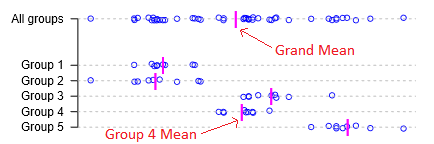
\includegraphics[width=\linewidth]{ANOVA.png}
\textbf{Hypotheses}: $H_{0}: \mu_{1} = \mu_{2} = \dots = \mu_{k}$ vs. $H_{1}: \bar{H}_{0}$\\
\textbf{Sum of Squares}:\\
Treatment SS:\\
$SS(T) = \sum_{i=1}^{k} \sum_{j=1}^{n_{i}} (\bar{X}_{i\cdot} - \bar{X}_{\cdot \cdot})^{2} = \sum_{i=1}^{k} n_{i} (\bar{X}_{i\cdot} - \bar{X}_{\cdot \cdot})^{2}$\\
Error SS:\\
$SS(E) = \sum_{i=1}^{k} \sum_{j=1}^{n_{i}} (X_{ij} - \bar{X}_{i\cdot})^{2} = \sum_{i=1}^{k} (n_{i} - 1) S_{i}^{2}$\\
Total SS:\\
$SS(TO) = \sum_{i=1}^{k} \sum_{j=1}^{n_{i}} (X_{ij} - \bar{X}_{\cdot \cdot})^{2} = SS(T) + SS(E)$\\
\textbf{Null Distributions of Sum of Squares Terms}:
$$\frac{SS(T)}{\sigma^{2}} \sim \chi^{2}_{k-1}; \quad \frac{SS(E)}{\sigma^{2}} \sim \chi^{2}_{n-k}; \quad \frac{SS(TO)}{\sigma^{2}} \sim \chi^{2}_{n-1}$$
\textbf{Test Statistic (F-test)}:
$$F = \frac{SS(T) / (k-1)}{SS(E) / (n-k)}$$
Under $H_{0}$, $F \sim \mbox{F}_{k-1, n-1}$, so since the numerator will be larger when $H_{0}$ is false reject $H_{0}$ for $F > c$.

{\color{magenta}\subsubsection*{Two Factor (Two Way) ANOVA}}
Assume $X_{ij} \sim N(\mu_{ij}, \sigma^{2})$. $\mu_{ij} = \mu + \alpha_{i} + \beta_{j}$. $\sum_{i=1}^{a} \alpha_{i} = 0$ and $\sum_{j=1}^{b} \beta_{j} = 0$. Take one observation from each combination of $a$ and $b$ ($n = ab$).\\
\textbf{Hypotheses}: $H_{0A}: \alpha_{1} = \alpha_{2} = \dots = \alpha_{k} = 0$ vs. $H_{1}: \bar{H}_{0}$\\
or $H_{0B}: \beta_{1} = \beta_{2} = \dots = \beta_{k} = 0$ vs. $H_{1}: \bar{H}_{0}$\\
\textbf{Means}:
$$\bar{X}_{\cdot \cdot} = \frac{1}{ab} \sum_{i=1}^{a} \sum_{j=1}^{b} X_{ij}; \quad \bar{X}_{i \cdot} = \frac{1}{b} \sum_{j=1}^{b} X_{ij}; \quad \bar{X}_{\cdot j} = \frac{1}{a} \sum_{i=1}^{a} X_{ij}$$
\textbf{Sum of Squares}:\\
$SS(A) = b \sum_{i=1}^{a} (\bar{X}_{i\cdot} - \bar{X}_{\cdot \cdot})^{2}$\\
$SS(B) = a \sum_{j=1}^{b} (\bar{X}_{\cdot j} - \bar{X}_{\cdot \cdot})^{2}$\\
Error SS:\\
$SS(E) = \sum_{i=1}^{a} \sum_{j=1}^{b} (X_{ij} - \bar{X}_{i\cdot} - \bar{X}_{\cdot j} + \bar{X}_{\cdot \cdot})^{2}$\\
Total SS:\\
$SS(TO) = SS(A) + SS(B) + SS(E)$\\
\textbf{Test Statistics (F-test)}:\\
The test statistics for $H_{0A}$ and $H_{0B}$ are:
$$F = \frac{SS(A) / (a-1)}{SS(E) / (a-1)(b-1)} \quad \mbox{ or } \quad \frac{SS(B) / (b-1)}{SS(E) / (a-1)(b-1)} > c$$
With $c$ from $\mbox{F}_{a-1, (a-1)(b-1)}$ or $\mbox{F}_{b-1, (a-1)(b-1)}$ respectively.

{\color{magenta}\subsubsection*{Two Factor ANOVA with Interaction Terms}}
Take samples over two factors, but $c$ samples for each factor pair. $\mu_{ij} = \mu + \alpha_{i} + \beta_{j} + \gamma_{ij}$.\\
\textbf{Hypotheses}: $H_{0A}: \alpha_{1} = \alpha_{2} = \dots = \alpha_{k} = 0$ vs. $H_{1}: \bar{H}_{0}$\\
or $H_{0B}: \beta_{1} = \beta_{2} = \dots = \beta_{k} = 0$ vs. $H_{1}: \bar{H}_{0}$\\
or $H_{0AB}: \gamma_{ij} = 0\ \forall\ i, j$ vs. $H_{1}: \bar{H}_{0}$\\
\textbf{Means}:
$$\bar{X}_{i j \cdot} = \frac{1}{c} \sum_{k=1}^{c} X_{ijk}; \quad \bar{X}_{i \cdot \cdot} = \frac{1}{bc} \sum_{j=1}^{b} \sum_{k=1}^{c} X_{ijk}$$
$$ \bar{X}_{\cdot j \cdot} = \frac{1}{ac} \sum_{i=1}^{a} \sum_{k=1}^{c} X_{ijk}; \quad \bar{X}_{\cdot \cdot \cdot} = \frac{1}{abc} \sum_{i=1}^{a} \sum_{j=1}^{b} \sum_{k=1}^{c} X_{ijk}$$
\textbf{Sum of Squares}:\\
$SS(A) = bc \sum_{i=1}^{a} (\bar{X}_{i \cdot \cdot} - \bar{X}_{\cdot \cdot \cdot})^{2}$\\
$SS(B) = ac \sum_{j=1}^{b} (\bar{X}_{\cdot j \cdot} - \bar{X}_{\cdot \cdot \cdot})^{2}$\\
$SS(AB) = c \sum_{i=1}^{a} \sum_{j=1}^{b} (\bar{X}_{i j \cdot} - \bar{X}_{i \cdot \cdot} - \bar{X}_{\cdot j \cdot} + \bar{X}_{\cdot \cdot \cdot})^{2}$\\
Error SS:\\
$SS(E) = \sum_{i=1}^{a} \sum_{j=1}^{b} \sum_{k=1}^{c} (X_{ijk} - \bar{X}_{i j \cdot})^{2}$\\
Total SS:\\
$SS(TO) = SS(A) + SS(B) + SS(AB) + SS(E)$\\
\textbf{Test Statistics (F-test)}:\\
The test statistics for $H_{0A}$ and $H_{0B}$ are:
$$F = \frac{SS(A) / (a-1)}{SS(E) / ab(c-1)} \quad \mbox{ or } \quad \frac{SS(B) / (b-1)}{SS(E) / ab(c-1)} > c$$
With $c$ from $\mbox{F}_{a-1, ab(c-1)}$ or $\mbox{F}_{b-1, ab(c-1)}$ respectively.\\
And for $H_{0AB}$ with $c$ from $\mbox{F}_{(a-1)(b-1), ab(c-1)}$:
$$F = \frac{SS(AB) / (a-1)(b-1)}{SS(E) / ab(c-1)} > c$$

{\color{magenta}\subsubsection*{Mean Squares / Mean Square Error}}
MSE is found by dividing the $SS(E)$ by its degrees of freedom.\\
{\color{blue} $\hat{\sigma}^{2} = MS(E)$ is an unbiased estimator for the variance.}

\subsection*{Goodness-of-fit Test ($\chi^{2}$)}
$O_{i}$ is the Observed count of data in class $i$, $E_{i}$ is the Expected count under $H_{0}$. Be careful to use the count and not the proportion. For $k$ classes:
$$Q_{k-1} = \sum_{i=1}^{k} \frac{(O_{i} - E_{i})^{2}}{E_{i}} \approx \chi^{2}_{k-1}$$
Since the numerator $(O_{i} - E_{i})^{2}$ will be larger when $H_{0}$ is false, we reject $H_{0}$ for $Q_{k-1} > c$, with $c$ from $\chi^{2}_{k-1}$.\\
\textbf{Two Classes $(k = 2)$}\\
Testing $H_{0}: p = p_{1}$ vs. $H_{1}: p \neq p_{1}$\\
\textbf{More than Two Classes $(k > 2)$}\\
Let $p_{1}, \dots, p_{k}$ define the proportions of a categorical distribution. $H_{0}: ``p_{1}, \dots, p_{k} \mbox{ do define the distribution}"$ vs. $H_{1}: \bar{H}_{0}$

\subsection*{Other Formulae}
\textbf{Sample Variance}\\
$s^2 = \frac{1}{n-1} \sum_{i=1}^{n} (x_{i}-\bar{x})^2 = \frac{1}{n-1} \left( \left( \sum_{i=1}^{n} x_{i}^2 \right) -n \bar{x}^2 \right)$\\
\textbf{Cramér-Rao Lower Bound}\\
The CR Lower Bound is the minimum possible variance of an estimator $\hat{\theta}$ of $\theta$. It is the asymptotic variance of the MLE.
\vspace{-0.2cm}
{\setlength{\mathindent}{0.5cm}
\begin{alignat*}{4}
    &\ell(\theta) = \ln L(\theta); &&\qquad U(\theta) &&= \frac{\partial \ell}{\partial \theta} &&\mbox{\quad (Score Function)}\\
    &V(\theta) = -\frac{\partial U}{\partial \theta}; &&\qquad I(\theta) &&= \mathbb{E}(V(\theta)) &&\mbox{\quad (Fisher Information)}\\
    &\mbox{Var}(\hat{\theta}) \geq \frac{1}{I(\theta)} && && &&\mbox{\quad (CR Lower Bound)}
\end{alignat*} \vspace{-0.5cm}}\\
\noindent \textbf{Gamma Function in Beta + $\gamma$ Distributions}\\
$\Gamma(n) = (n-1)!$
\end{multicols*}
\end{document}